\documentclass{article}

\usepackage[utf8x]{inputenc}
\usepackage[frenchb]{babel}
\usepackage[T1]{fontenc}
\usepackage{lmodern}
\usepackage{fullpage}
\usepackage{graphicx}
\usepackage{epstopdf}
\usepackage{caption}
\usepackage{subcaption}
\usepackage{multirow}

% Math symbols
\usepackage{amsmath}
\usepackage{amssymb}
\usepackage{amsthm}

% Numbers and units
\usepackage[squaren, Gray]{SIunits}
\usepackage{sistyle}
\usepackage[autolanguage]{numprint}
%\usepackage{numprint}
\newcommand\si[2]{\numprint[#2]{#1}}
\newcommand\np[1]{\numprint{#1}}

\DeclareMathOperator{\newdiff}{d} % use \dif instead
\newcommand{\dif}{\newdiff\!}
\newcommand{\fpart}[2]{\frac{\partial #1}{\partial #2}}
\newcommand{\ffpart}[2]{\frac{\partial^2 #1}{\partial #2^2}}
\newcommand{\fdpart}[3]{\frac{\partial^2 #1}{\partial #2\partial #3}}
\newcommand{\fdif}[2]{\frac{\dif #1}{\dif #2}}
\newcommand{\ffdif}[2]{\frac{\dif^2 #1}{\dif #2^2}}
\newcommand{\constant}{\ensuremath{\mathrm{cst}}}

\title{Rapport}
\author{Benoît Legat}

\begin{document}

\maketitle

\section{Resources}
Mettez ici ce que vous trouvez intéressant
\begin{itemize}
  \item Montre comment trouver l'angle et la longueur en comparant Cepstral (mieux pour la longueur et mieux pour l'angle quand la longueur est petite (donc plus pour la caméra que pour le train)) et Radon (mieux pour l'angle avec une grande longueur donc pour le train) et Steerable filters (pourri) \cite{krahmer2006blind}.
  \item Explication de Radon \cite{oliveira2007blind}.
  \item Angle: En gros, il faut voir l'angle des lignes qui sont dans le spectre pour ça il y a: Hough, Radon et Gabor et il conseille Gabor.
    Longueur: Il conseille d'utiliser un Cepstral modifié qu'on utilise et qui marche bien mieux \cite{Deshpande2014606}.
\end{itemize}

\section{Quelques résolution avec PSF connue}

\begin{figure}[!ht]
  \centering
  \begin{subfigure}[b]{0.45\textwidth}
    \includegraphics[width=\textwidth]{../matlab/start-nonoise.png}
    \caption{Image de départ}
    \label{fig:start-nonoise}
  \end{subfigure}
  \begin{subfigure}[b]{0.45\textwidth}
    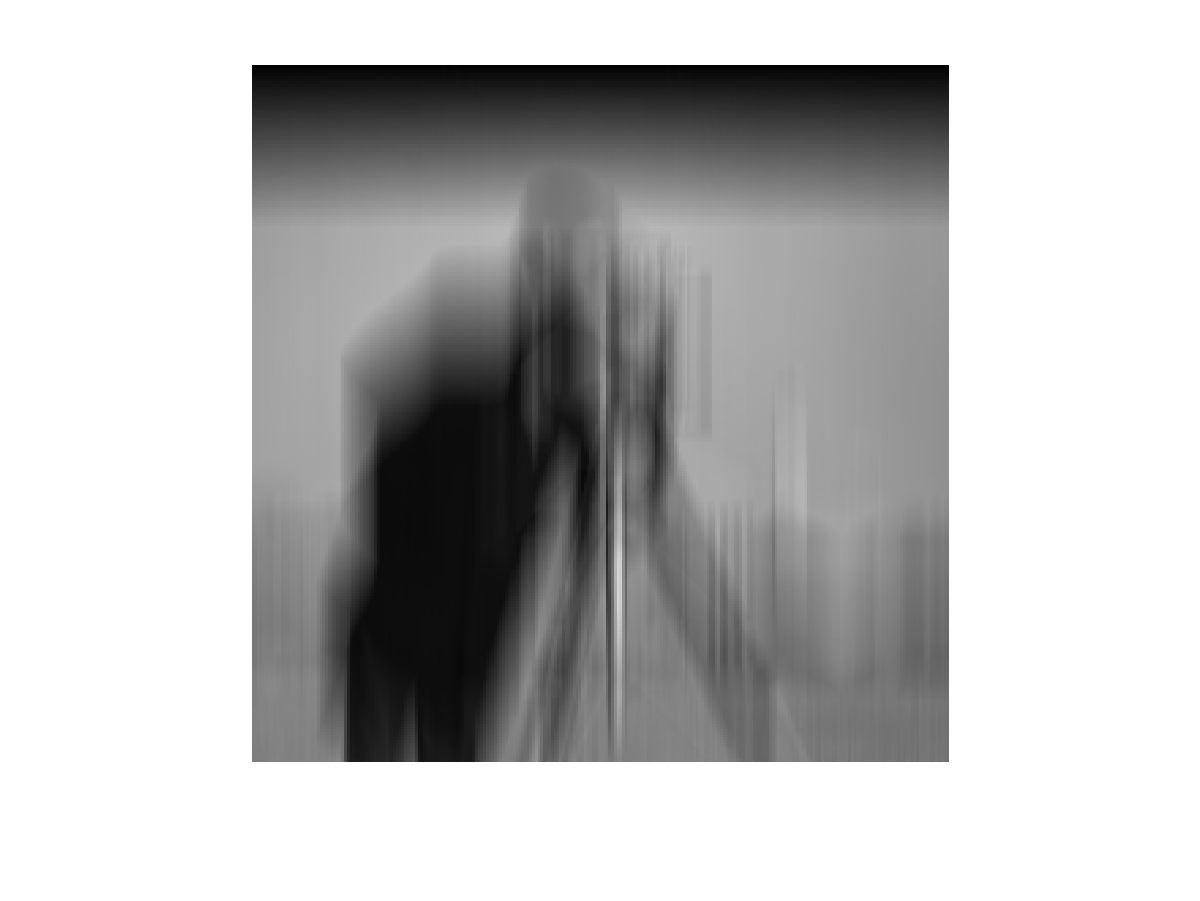
\includegraphics[width=\textwidth]{../matlab/matb-nonoise.png}
    \caption{Image flouté par matrice}
    \label{fig:matb-nonoise}
  \end{subfigure}%
  \begin{subfigure}[b]{0.45\textwidth}
    \includegraphics[width=\textwidth]{../matlab/psfb-nonoise.png}
    \caption{Image floutée par PSF}
    \label{fig:psfb-nonoise_explicite_lambda}
  \end{subfigure}
  \begin{subfigure}[b]{0.45\textwidth}
    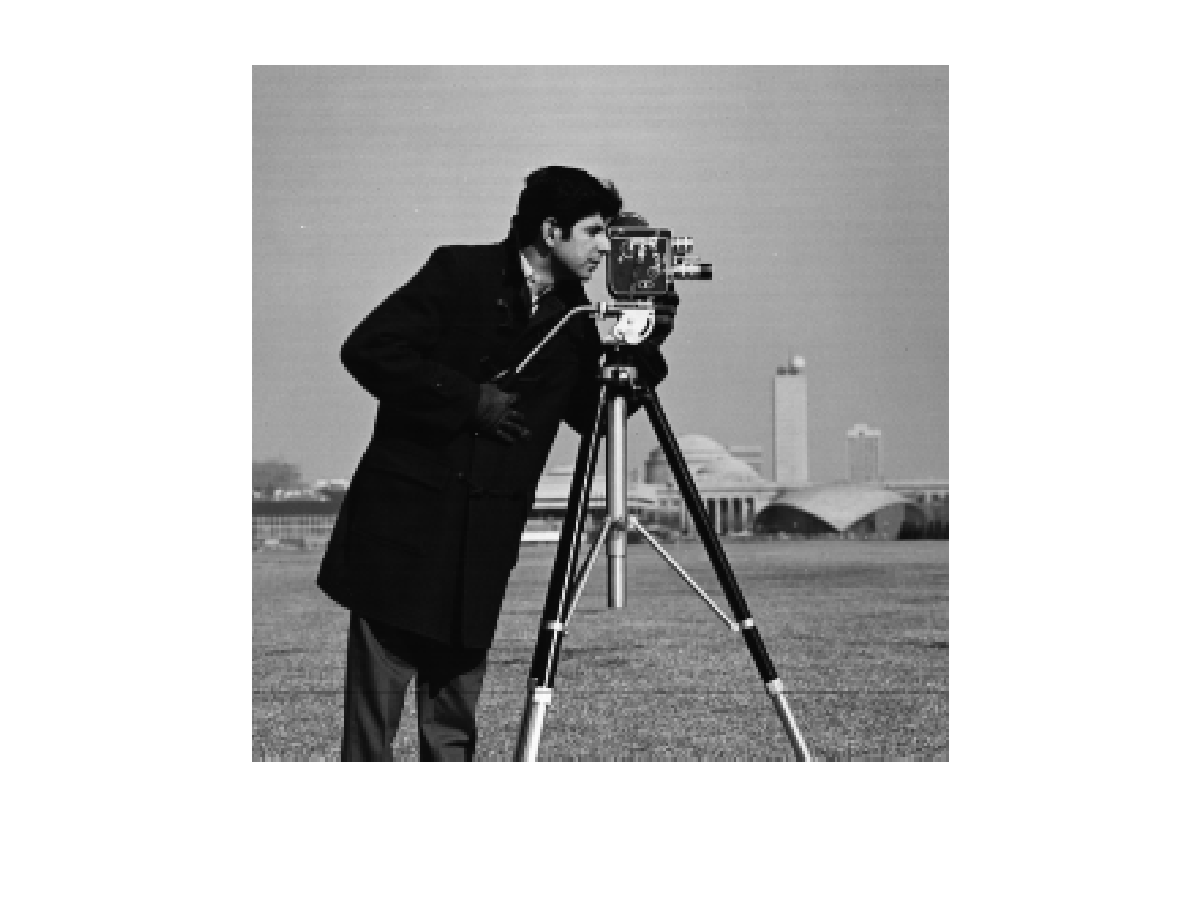
\includegraphics[width=\textwidth]{../matlab/direct-nonoise.png}
    \caption{Image déflouté par méthode directe}
    \label{fig:direct-nonoise}
  \end{subfigure}
  \begin{subfigure}[b]{0.45\textwidth}
    \includegraphics[width=\textwidth]{../matlab/lucy-nonoise.png}
    \caption{Image défloutée par Lucy-Richardson}
    \label{fig:lucy-nonoise}
  \end{subfigure}
  \caption{Résultats pour une image sans noise}
  \label{fig:nonoise}
\end{figure}

\begin{figure}[!ht]
  \centering
  \begin{subfigure}[b]{0.45\textwidth}
    \includegraphics[width=\textwidth]{../matlab/start-noise-g10.png}
    \caption{Image de départ}
    \label{fig:start-noise-g10}
  \end{subfigure}
  \begin{subfigure}[b]{0.45\textwidth}
    \includegraphics[width=\textwidth]{../matlab/matb-noise-g10.png}
    \caption{Image flouté par matrice}
    \label{fig:matb-noise-g10}
  \end{subfigure}%
  \begin{subfigure}[b]{0.45\textwidth}
    \includegraphics[width=\textwidth]{../matlab/psfb-noise-g10.png}
    \caption{Image floutée par PSF}
    \label{fig:psfb-noise-g10_explicite_lambda}
  \end{subfigure}
  \begin{subfigure}[b]{0.45\textwidth}
    \includegraphics[width=\textwidth]{../matlab/direct-noise-g10.png}
    \caption{Image déflouté par méthode directe}
    \label{fig:direct-noise-g10}
  \end{subfigure}
  \begin{subfigure}[b]{0.45\textwidth}
    \includegraphics[width=\textwidth]{../matlab/lucy-noise-g10.png}
    \caption{Image défloutée par Lucy-Richardson}
    \label{fig:lucy-noise-g10}
  \end{subfigure}
  \caption{Résultats pour une image avec noise gaussien}
  \label{fig:noise-g10}
\end{figure}

\begin{figure}[!ht]
  \centering
  \begin{subfigure}[b]{0.45\textwidth}
    \includegraphics[width=\textwidth]{../matlab/start-noise-poisson.png}
    \caption{Image de départ}
    \label{fig:start-noise-poisson}
  \end{subfigure}
  \begin{subfigure}[b]{0.45\textwidth}
    \includegraphics[width=\textwidth]{../matlab/matb-noise-poisson.png}
    \caption{Image flouté par matrice}
    \label{fig:matb-noise-poisson}
  \end{subfigure}%
  \begin{subfigure}[b]{0.45\textwidth}
    \includegraphics[width=\textwidth]{../matlab/psfb-noise-poisson.png}
    \caption{Image floutée par PSF}
    \label{fig:psfb-noise-poisson_explicite_lambda}
  \end{subfigure}
  \begin{subfigure}[b]{0.45\textwidth}
    \includegraphics[width=\textwidth]{../matlab/direct-noise-poisson.png}
    \caption{Image déflouté par méthode directe}
    \label{fig:direct-noise-poisson}
  \end{subfigure}
  \begin{subfigure}[b]{0.45\textwidth}
    \includegraphics[width=\textwidth]{../matlab/lucy-noise-poisson.png}
    \caption{Image défloutée par Lucy-Richardson}
    \label{fig:lucy-noise-poisson}
  \end{subfigure}
  \caption{Résultats pour une image avec noise poisson}
  \label{fig:noise-poisson}
\end{figure}

\bibliographystyle{plain}
\bibliography{biblio}

\end{document}
